\section{Model Validation}
\label{sec:model_validation}

This compares simulated data from our model with empirical data from Germany. We at
observed infections, fatality rates, the spread of the B117 mutation, vaccinations and
rapid test demands. Where available we do not only look at aggregated statistics but
also analyze the model fit for age groups.

\textcolor{red}{summarize the fit; Some of this needs to go in the appendix. I suggest the age group and federal state fit goes there???}


\subsection{Observed Infections}
\label{sub:in_sample_fit}

% Despite fitting only four infection probabilities, the in-sample fit is very good. The
% best fit is achieved in the largest age groups. This is so mechanically, because we
% weigh the deviations between simulated and observed infection rates by group sizes.
% The worst fit is achieved for the 80 to 100 years old. There are three reasons for
% this: Firstly, we only model private households at the moment, meaning that nursing
% homes are not part of the synthetic population we simulate. Since community housing
% residents are part of the German Mikrozensus \citep{FDSAeDBUDL2018} which forms the
% basis for our synthetic population, we can and plan to include community housing
% residents in the near future. Secondly, the elderly, especially nursing home
% residents, are tested more often than the general population leading to more cases
% being detected in this age group. We are currently working to include age-variant
% testing strategies, using \href{https://ars.rki.de/Content/COVID19/Main.aspx}{data by
% the RKI} \citep{Seifried2020}.



\begin{figure}[ht]
\centering
  % 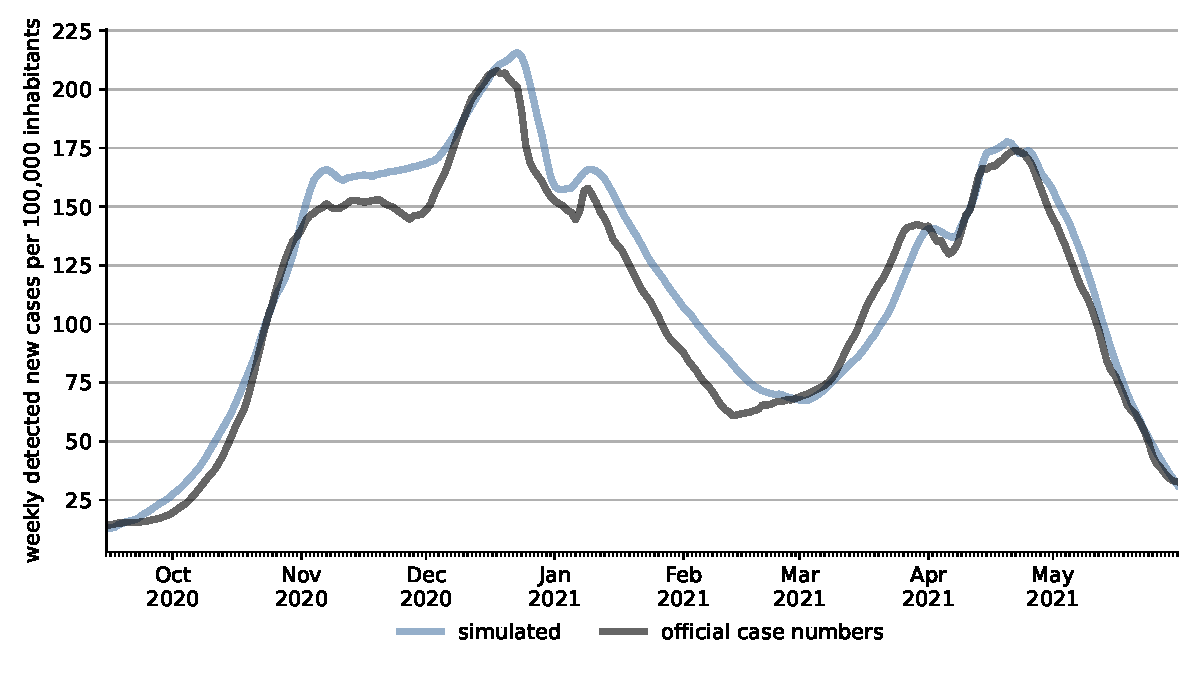
\includegraphics[width=\textwidth]{../figures/results/figures/scenario_comparisons/combined_fit/full_new_known_case}
\caption{Simulated and Empirical Infections}
\figurenotes{The figure shows the weekly incidence rates per 100,000 people for the reported versus the simulated infections rates.}
\label{fig:aggregated_fit2}
\end{figure}



\begin{figure}[ht]
\centering
  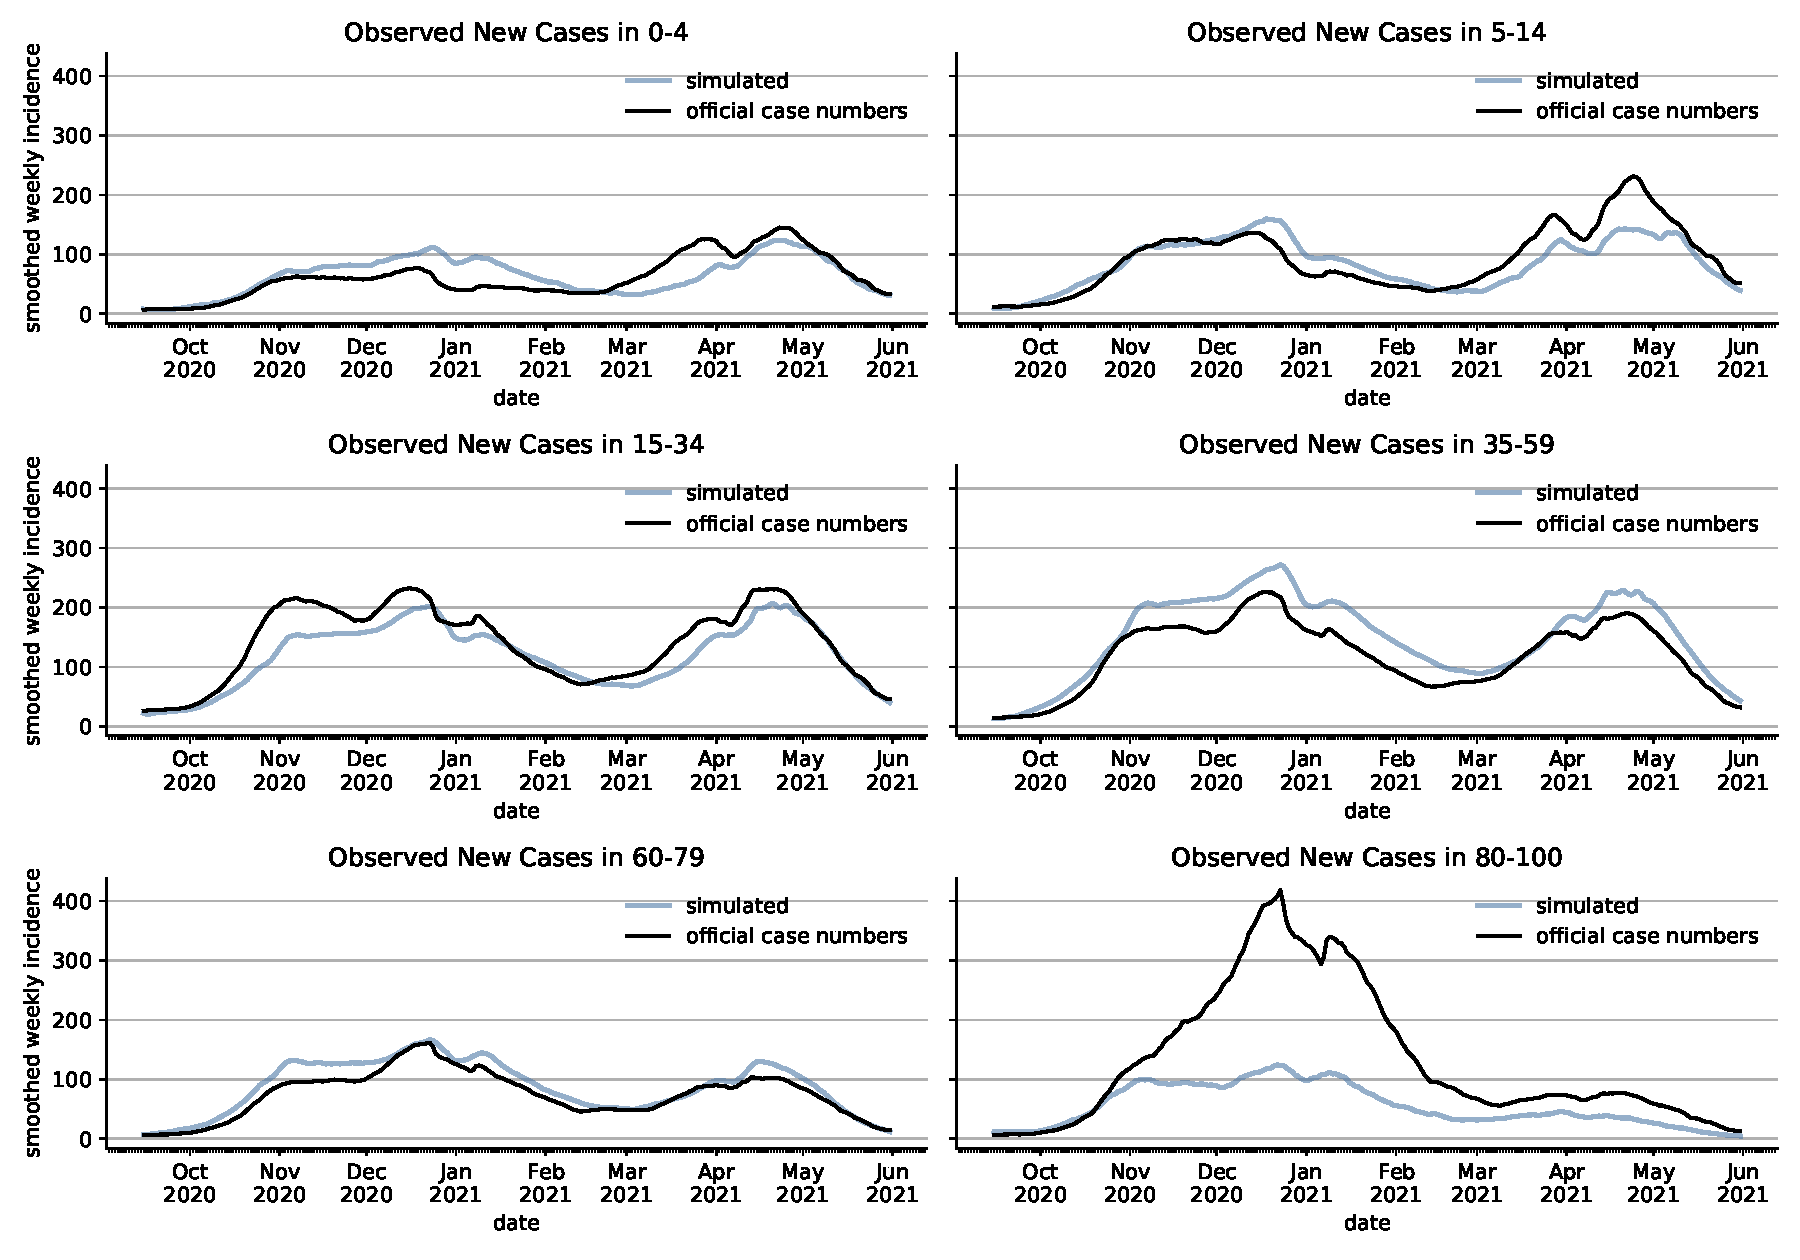
\includegraphics[width=\textwidth]{../figures/results/figures/incidences_by_group/age_group_rki/full_combined_baseline_new_known_case}
\caption{Simulated and Empirical Infections by Age Group}
\figurenotes{The figure shows the weekly incidence rates per 100,000 people for the reported versus the simulated infections rates for different age groups.}
\label{fig:age_group_fit}
\end{figure}


\begin{figure}[ht]
\centering
  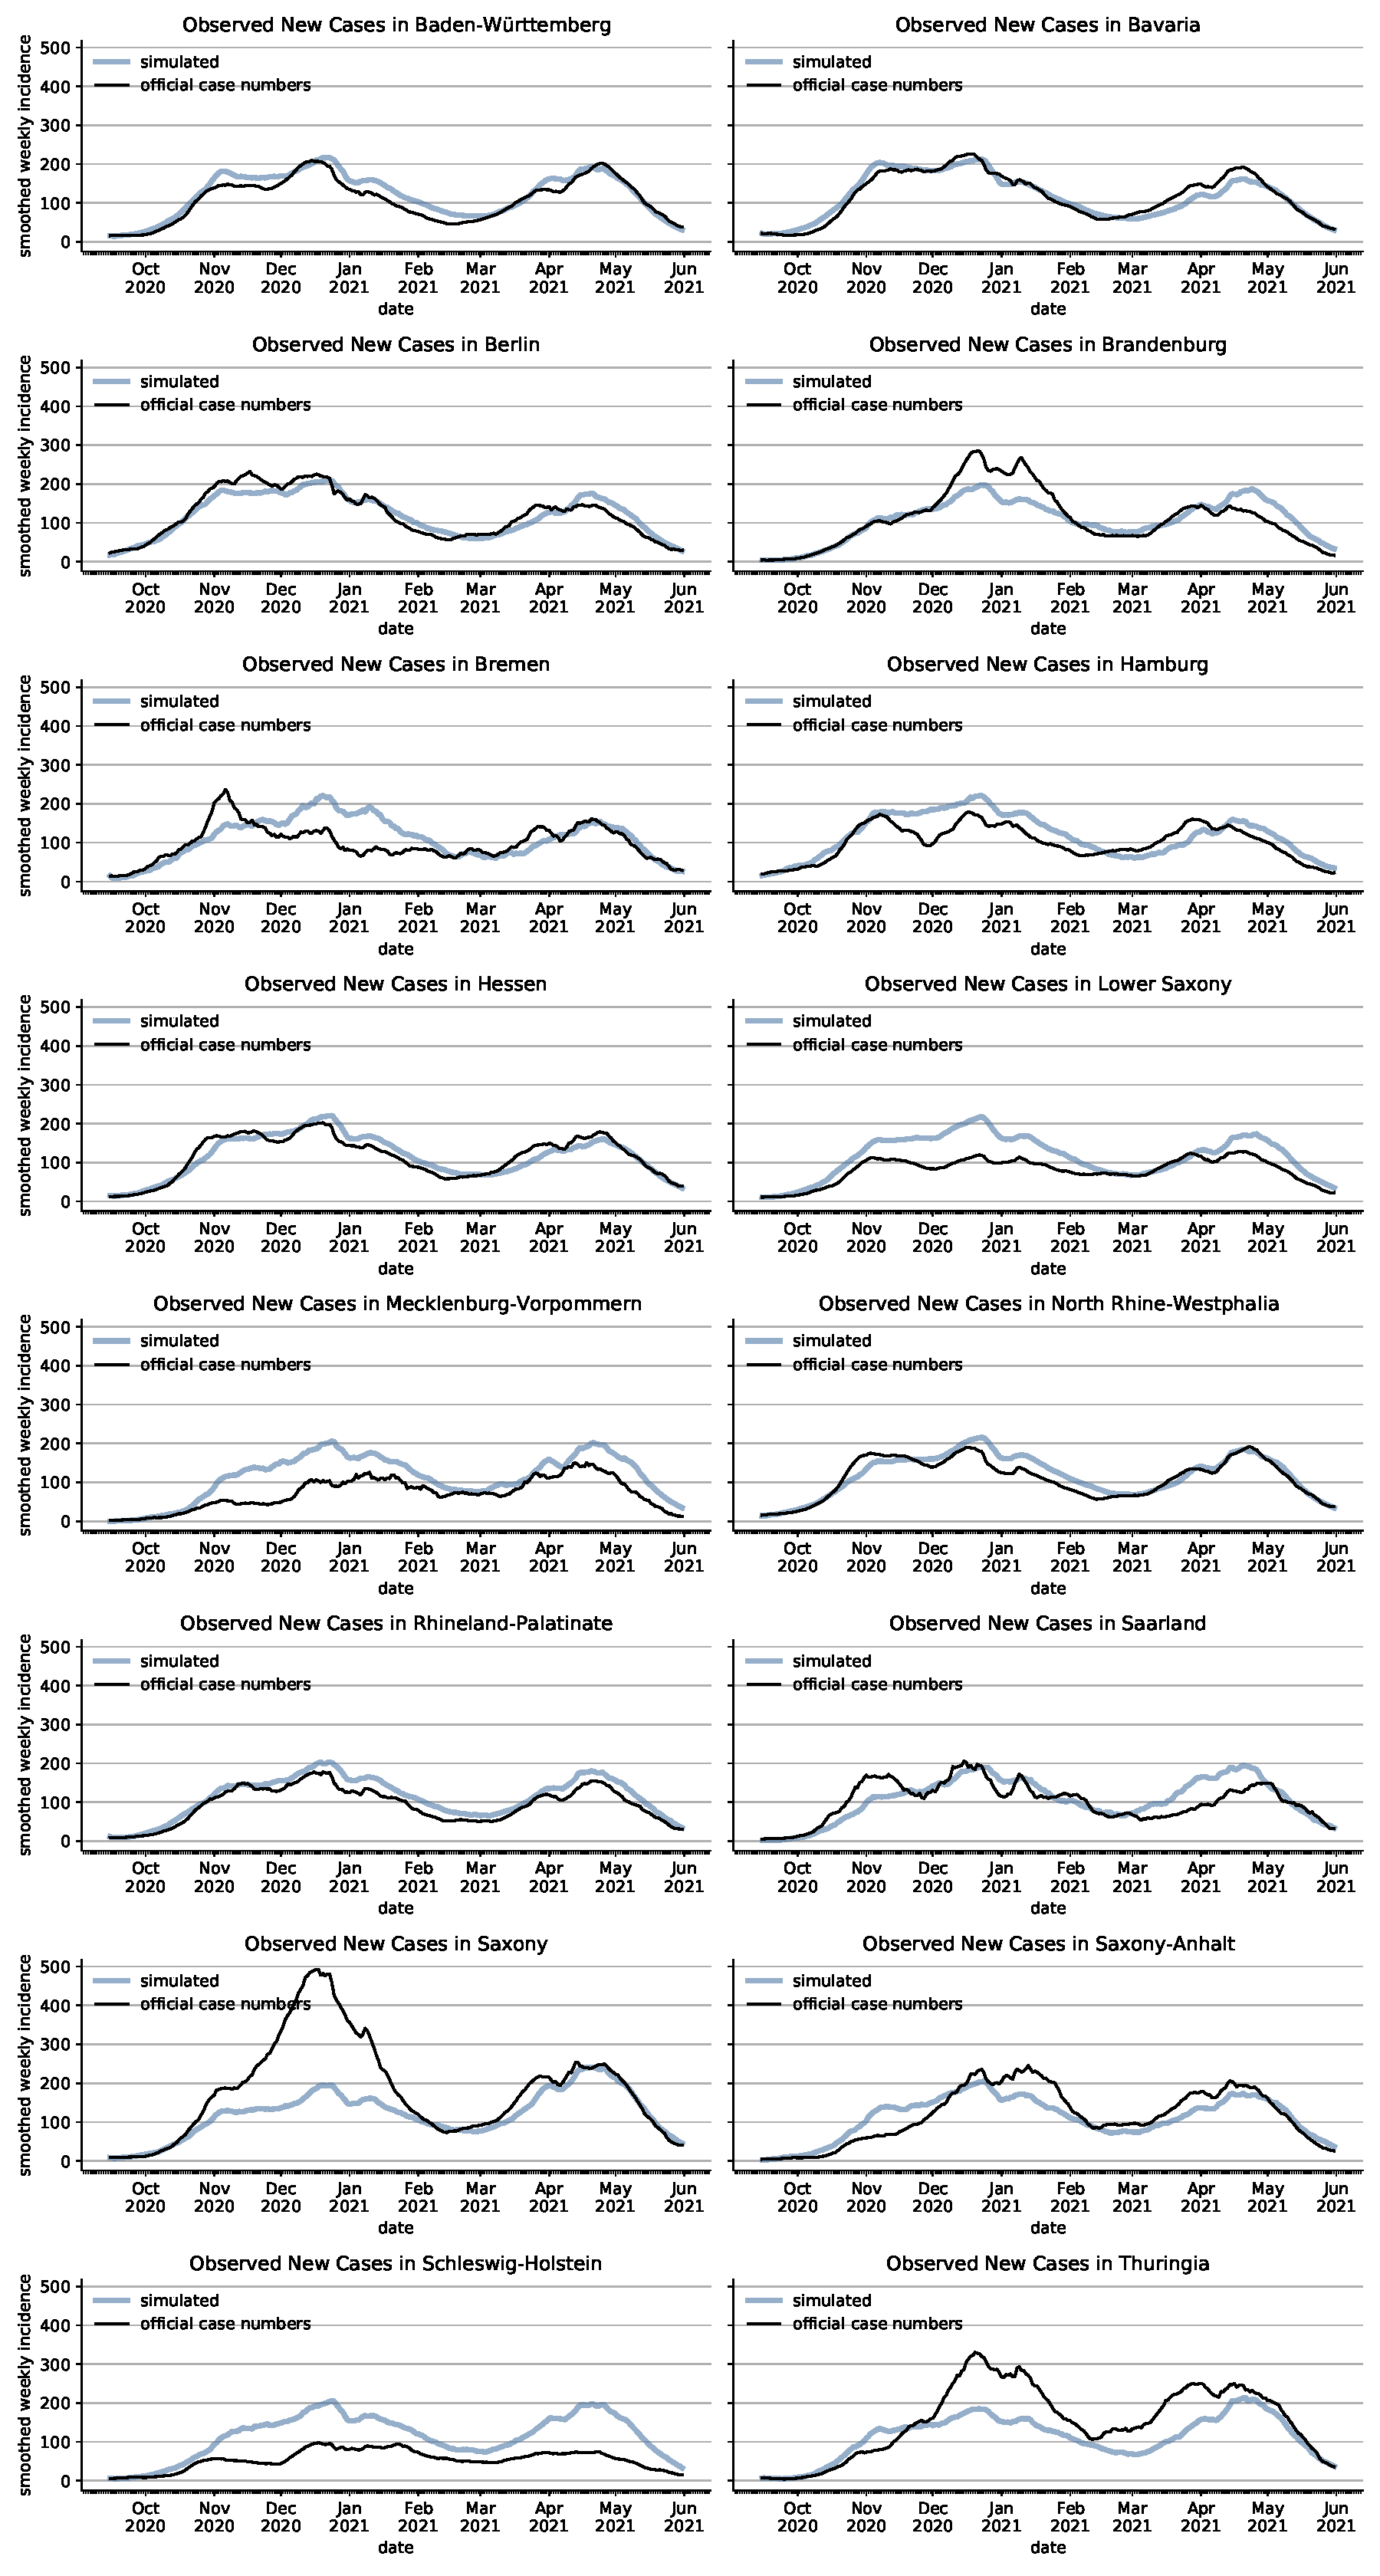
\includegraphics[width=\textwidth]{../figures/results/figures/incidences_by_group/state/full_combined_baseline_new_known_case}
\caption{Simulated and Empirical Infections by Federal State}
\figurenotes{The figure shows the weekly incidence rates per 100,000 people for the reported versus the simulated infections rates for different federal states.}
\label{fig:state_fit}
\end{figure}



\FloatBarrier


\section{The Spread of the B117 Mutation}


\textcolor{red}{We don't have this figure in the repo yet, but the fit is perfect}



\FloatBarrier

\subsection{Out-of-Sample Fit}
\label{sub:out_of_sample_fit}

We can assess the out-of-sample fit by projecting the effect of the lockdown light and
comparing it to case numbers until mid of November. It is important to note that this is
not just a simple extrapolation of a time trend because the lockdown light only started
after the estimation period. The out-of-sample fit can be assessed in
Figure~\ref{fig:out-of-sample-fit}.

\begin{figure}[!tp]
    \centering
    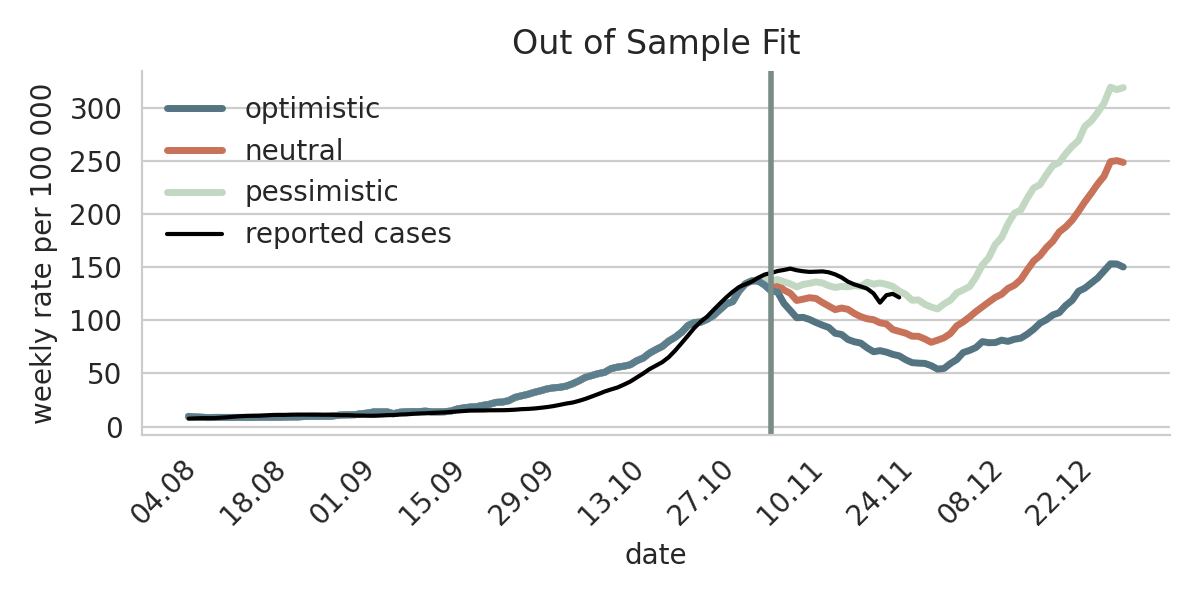
\includegraphics[width=\textwidth]{../figures/out_of_sample_validation}
    \caption{Predicted effect of the "Lockdown Light" on infection rates.}
    \label{fig:out-of-sample-fit}
    \figurenotes{For the time period until the beginning of November, the figure shows
        the weekly incidence rates of infections per 100,000 people from reported
        (black) versus simulated (blue) data. With the start of November, the
        projections of the three scenarios, optimistic (blue), neutral (red), and
        pessimistic (mint green), are shown until the beginning of the Christmas
        holidays. The actual incidence rates (black) are reported until the 24th
        November.}
\end{figure}

The model correctly predicts the effect of the lockdown light with reasonable accuracy.
In particular, the actual case numbers are between our neutral and pessimistic
projection. The plot also shows that ending the lockdown light on November 30, as was
originally planned, would lead to an explosive growth in case numbers in all scenarios.
